\section{CSGCN-IS}\label{sec:csgcn_is}
This section describes the first of our two proposed models, Context and Side-information GCN with Item-Splitting (CSGCN-IS), which is a GCN that incorporates side-information in the graph and considers context as an embedding that is used as a modifier for an item.

\subsection{Model intuition}\label{subsec:csgcn_is_intuition}
Before diving into the details of how CSGCN-IS is modeled, let us examine the intuition behind it.
The goal is to construct a model that can generate a top-$k$ list of recommendations for a user.
To do this, we start by expressing the available information in a graph.
This mainly includes interactions between users and items.
However, since most RS datasets are sparse, we want to see if we can alleviate this problem by further connecting user and item nodes, to improve the collaborative signals in the model.
To do this, we utilize the fact that most datasets include some side-information about users and items, which can be used for further connections by its addition as nodes in the graph.\\
Besides side-information, we need to reason about how to express context in the model.
In this model, we express context by simplifying it to be an embedding that is used as a modifier to an item to signify whether the item is popular in a given context or not.
For example, we may learn that indoor activities are generally more popular on a rainy day.
This can be learned by the model through sampling user interactions in various contexts from the ground truth.
For the user and context of the positive sampled interaction, we see that they interacted with a given item, which should make the item more likely to be recommended in that context.
A negative interaction is also sampled for the same user and context, which should make the item less likely to be recommended for that context through training, further detailed in \Cref{subsec:csgcn_is_training}.
With this intuition, we will now detail how this is implemented in the CSGCN-IS model.

\subsection{Model architecture}\label{subsec:csgcn_is_model_architecture}
The CSGCN models are based on the observations made in SGC \cite{SimplifyingGCN} and the LightGCN model \cite{LightGCN} about simplifying the models to a linear model.
To facilitate the model architecture, each node in the graph is represented by a low-dimensional vector called an embedding.
By doing this, the model can learn the nodes' properties and capture them in the embeddings.
The model consists of four parts: Input, graph convolution layers, layer combination, and a prediction function.\\
The input is represented as a quadripartite graph consisting of users, items, user side-information, and item side-information.
This graph is used as the input for the graph convolution layers, which serve to capture higher-order connectivities between the nodes in the graph.
Each convolutional layer is stacked on top of the previous layer, such that each layer captures information from nodes that are further away from the central node.
Having passed through $L$ convolution layers, we are left with an embedding representation of each node for each layer, which is then passed to the layer combination function, taking a weighted sum of each representation to generate a final representation for each node.\\
Finally, these combined representations of users and items are passed to a prediction function along with a context embedding to calculate a score for the given user, item, and context combination as described in \Cref{subsec:csgcn_is_intuition}.\\
These predicted scores are used to generate a top-$k$ list of recommended items for a user in the given context.\\
In the following sections we will further explain how each of these four parts of the model work.



%\begin{figure}[hbt!]
    %\hspace*{-0.1cm}
%   \centering
%   \small  
%   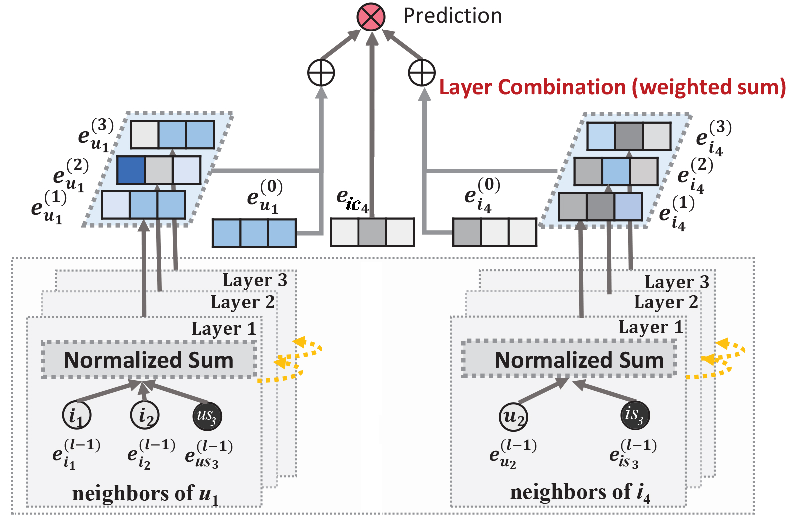
\includegraphics[width=0.48\textwidth]{figures/CSGCN.pdf}\vspace{-5pt}
%   \caption{An illustration of CSGCN-IS model architecture. User and item neighbors are illustrated as bright nodes, and side-information as dark nodes. In the layer combination, we sum over the embeddings at each layer to obtain the final representations.}\vspace{-10pt}
%   \label{fig:csgcn_is_model}
%\end{figure}
%The model itself is very similar to LightGCN.
%It is, however, important to note that the neighboring nodes for users now include side-information for users and not only items, which can be seen in each of the layers now receiving a normalized sum of both items and user side-information, rather than just the normalized sum of items.
%The same goes for the neighbors of items.

\subsection{Adjacency matrix}\label{subsec:csgcn_is_adj_mat}
As described in \Cref{sec:preliminaries}, GCNs used for CF recommendation typically employ a bipartite graph structure to represent the user-item interactions.
In CSGCN-IS the extended graph now contains users, items and edges as well as the set of user side-information nodes $US$ and the set of item side-information nodes $IS$.
This allows for the incorporation of side-information in the model, whereas context is later included in the prediction function defined in \autoref{subsec:csgcn_is_score_prediction}.
This graph extension can be seen on \Cref{fig:quadripartite-graph}.
It should be noted that the distinct sets cannot be self-connected, and edges can only exist between adjacent sets.
Formally, we let $G$ be a graph consisting of a set of edges $E$, and vertices $V$, where $V = US \cup U \cup I \cup IS$.
$$E_{US} \subseteq \{ (x,y) | \: x \in US, \: y \in U  \}$$
$$E_U \subseteq \{ (x,y) | \: x \in U, \: y \in US \cup I \}$$
$$E_I \subseteq \{ (x,y) | \: x \in I, \: y \in U \cup IS \}$$
$$E_{IS} \subseteq \{ (x,y) | \: x \in IS, \: y \in I  \}$$
$$E = E_{US} \cup E_{U} \cup E_{I} \cup E_{IS} $$

\begin{figure}[h]
\begin{tikzpicture}[thick,
    every node/.style={draw,circle},
    inode/.style={fill=myred},
    unode/.style={fill=myblue},
    isnode/.style={fill=green},
    usnode/.style={fill=yellow},
    every fit/.style={ellipse,draw,inner sep=-2pt,text width=1.3cm},
    shorten >= 3pt,shorten <= 3pt
  ]
  
  % the vertices of US
  \begin{scope}[start chain=going below,node distance=7mm]
  \foreach \i in {us1,us2,us3}
    \node[usnode,on chain] (\i) [] {};
  \end{scope}
  
  % the vertices of U
  \begin{scope}[xshift=2cm,start chain=going below,node distance=7mm]
  \foreach \i in {u1,u2,u3}
    \node[unode,on chain] (\i) [] {};
  \end{scope}
  
  % the vertices of I
  \begin{scope}[xshift=4cm,start chain=going below,node distance=7mm]
  \foreach \i in {i1,i2,i3,i4}
    \node[inode,on chain] (\i) [] {};
  \end{scope}
  
  % the vertices of IS
  \begin{scope}[xshift=6cm,start chain=going below,node distance=7mm]
  \foreach \i in {is1,is2,is3,is4}
    \node[isnode,on chain] (\i) [] {};
  \end{scope}
  
  % the set U
  \node [myblue,fit=(u1) (u3),label=above:$U$] {};
  % the set I
  \node [myred,fit=(i1) (i4),label=above:$I$] {};
  % the set US
  \node [yellow,fit=(us1) (us3),label=above:$US$] {};
  % the set IS
  \node [green,fit=(is1) (is4),label=above:$IS$] {};
  
  % the edges
  \draw (us1) -- (u2);
  \draw (us2) -- (u1);
  \draw (us3) -- (u3);
  \draw (us3) -- (u1);
  \draw (u1) -- (i3);
  \draw (u2) -- (i2);
  \draw (u3) -- (i1);
  \draw (u2) -- (i4);
  \draw (i1) -- (is3);
  \draw (i2) -- (is1);
  \draw (i3) -- (is1);
  \draw (i4) -- (is4);
  \draw (i3) -- (is2);
\end{tikzpicture}
\caption{Example of the quadripartite graph structure used for CSGCN-IS.}
\label{fig:quadripartite-graph}
\end{figure}
The quadripartite graph can be represented as an adjacency matrix $A \in \mathbb{R}^{|U|\times|I|\times|US| \times |IS|}$.
An entry is $1$ if the user has interacted with the item, if the item has the given side-information or if a user has the given side-information, and $0$ if none of these are true.
$A$ consists of the rating sub-matrix $R$ and its transpose $R^T$, as well as sub-matrices containing $US$, $IS$, and their transposes, as seen on \Cref{csgcn_is_adj_mat}.
\begin{equation}\label{csgcn_is_adj_mat}
    \begin{bmatrix}
    0 & R & US & 0\\
    R^T & 0 & 0 & IS\\
    US^T & 0 & 0 & 0 \\
    0 & IS^T & 0 & 0
    \end{bmatrix}
\end{equation}
Since there are no direct interactions between users and other users, the first quadrant is a zero-matrix of size $|U|\times|U|$ where $|U|$ is the amount of users in the dataset.
This goes for all the zero matrices seen on $A$, making it mostly sparse.
Adding the side-information to the adjacency matrix allows us to express the connections between users and items and their side-information in the graph, allowing it to be used in order to gain higher-order connectivity in the convolution layers.\\
It is worth noting that, unlike traditional GCNs, CSGCN does not utilize self-connections since the layer combination performed after the convolution layers captures the same effect as self-connections through the 0th layer \cite{LightGCN}.

\subsection{Convolution layers}\label{subsec:csgcn_is_conv_layer}
A major part of the model is the convolution layer where the user and item embeddings are propagated with information about their neighbor nodes' representations by using an aggregation function, which in this case is a normalized sum.
Neighbor nodes for users are item nodes and user side-information nodes, and for items the neighbors are user nodes and item side-information nodes, which can be seen on \Cref{fig:quadripartite-graph}.
For each additional layer, information is passed from nodes that are further away from a central node, illustrated on \Cref{fig:aggregation-for-layers}.
\begin{figure}[h]
    \centering
    \tikzset{every picture/.style={line width=0.75pt}} %set default line width to 0.75pt        
    
    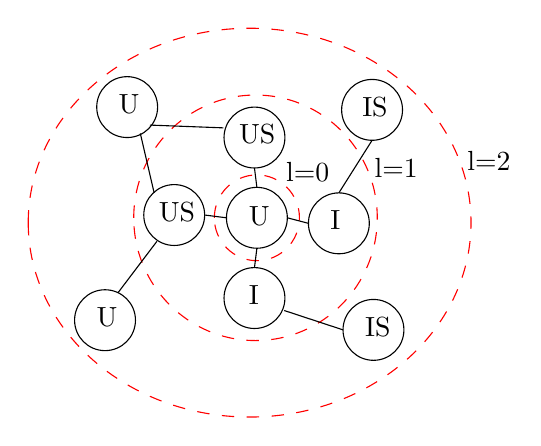
\begin{tikzpicture}[x=0.5pt,y=0.5pt,yscale=-1,xscale=1]
    %uncomment if require: \path (0,300); %set diagram left start at 0, and has height of 300
    
    %Flowchart: Connector [id:dp27406580802635316] 
    \draw   (290.75,139) .. controls (290.75,126.85) and (300.6,117) .. (312.75,117) .. controls (324.9,117) and (334.75,126.85) .. (334.75,139) .. controls (334.75,151.15) and (324.9,161) .. (312.75,161) .. controls (300.6,161) and (290.75,151.15) .. (290.75,139) -- cycle ;
    %Flowchart: Connector [id:dp597318920352127] 
    \draw   (289,81) .. controls (289,68.85) and (298.85,59) .. (311,59) .. controls (323.15,59) and (333,68.85) .. (333,81) .. controls (333,93.15) and (323.15,103) .. (311,103) .. controls (298.85,103) and (289,93.15) .. (289,81) -- cycle ;
    %Flowchart: Connector [id:dp057928841134587516] 
    \draw   (350,143) .. controls (350,130.85) and (359.85,121) .. (372,121) .. controls (384.15,121) and (394,130.85) .. (394,143) .. controls (394,155.15) and (384.15,165) .. (372,165) .. controls (359.85,165) and (350,155.15) .. (350,143) -- cycle ;
    %Flowchart: Connector [id:dp11200641374570286] 
    \draw   (289,197) .. controls (289,184.85) and (298.85,175) .. (311,175) .. controls (323.15,175) and (333,184.85) .. (333,197) .. controls (333,209.15) and (323.15,219) .. (311,219) .. controls (298.85,219) and (289,209.15) .. (289,197) -- cycle ;
    %Flowchart: Connector [id:dp5153973147602738] 
    \draw   (231,137) .. controls (231,124.85) and (240.85,115) .. (253,115) .. controls (265.15,115) and (275,124.85) .. (275,137) .. controls (275,149.15) and (265.15,159) .. (253,159) .. controls (240.85,159) and (231,149.15) .. (231,137) -- cycle ;
    %Flowchart: Connector [id:dp6230129861696904] 
    \draw   (197,59) .. controls (197,46.85) and (206.85,37) .. (219,37) .. controls (231.15,37) and (241,46.85) .. (241,59) .. controls (241,71.15) and (231.15,81) .. (219,81) .. controls (206.85,81) and (197,71.15) .. (197,59) -- cycle ;
    %Flowchart: Connector [id:dp11627558541491778] 
    \draw   (181,213) .. controls (181,200.85) and (190.85,191) .. (203,191) .. controls (215.15,191) and (225,200.85) .. (225,213) .. controls (225,225.15) and (215.15,235) .. (203,235) .. controls (190.85,235) and (181,225.15) .. (181,213) -- cycle ;
    %Flowchart: Connector [id:dp012014051199046416] 
    \draw   (374,61) .. controls (374,48.85) and (383.85,39) .. (396,39) .. controls (408.15,39) and (418,48.85) .. (418,61) .. controls (418,73.15) and (408.15,83) .. (396,83) .. controls (383.85,83) and (374,73.15) .. (374,61) -- cycle ;
    %Flowchart: Connector [id:dp025105219979997373] 
    \draw   (375,220) .. controls (375,207.85) and (384.85,198) .. (397,198) .. controls (409.15,198) and (419,207.85) .. (419,220) .. controls (419,232.15) and (409.15,242) .. (397,242) .. controls (384.85,242) and (375,232.15) .. (375,220) -- cycle ;
    %Flowchart: Connector [id:dp28306483017107376] 
    \draw  [color={rgb, 255:red, 255; green, 0; blue, 0 }  ,draw opacity=1 ][dash pattern={on 4.5pt off 4.5pt}] (282,139) .. controls (282,121.88) and (295.77,108) .. (312.75,108) .. controls (329.73,108) and (343.5,121.88) .. (343.5,139) .. controls (343.5,156.12) and (329.73,170) .. (312.75,170) .. controls (295.77,170) and (282,156.12) .. (282,139) -- cycle ;
    %Flowchart: Connector [id:dp22791557868185153] 
    \draw  [color={rgb, 255:red, 255; green, 0; blue, 0 }  ,draw opacity=1 ][dash pattern={on 4.5pt off 4.5pt}] (223.75,139) .. controls (223.75,90) and (263.15,50.28) .. (311.75,50.28) .. controls (360.35,50.28) and (399.75,90) .. (399.75,139) .. controls (399.75,188) and (360.35,227.72) .. (311.75,227.72) .. controls (263.15,227.72) and (223.75,188) .. (223.75,139) -- cycle ;
    %Flowchart: Connector [id:dp946514520124221] 
    \draw  [color={rgb, 255:red, 255; green, 0; blue, 0 }  ,draw opacity=1 ][dash pattern={on 4.5pt off 4.5pt}] (147.5,142.5) .. controls (147.5,64.9) and (219.13,2) .. (307.5,2) .. controls (395.87,2) and (467.5,64.9) .. (467.5,142.5) .. controls (467.5,220.1) and (395.87,283) .. (307.5,283) .. controls (219.13,283) and (147.5,220.1) .. (147.5,142.5) -- cycle ;
    %Straight Lines [id:da566741285857424] 
    \draw    (235.5,72) -- (288.5,74) ;
    %Straight Lines [id:da31194843739323463] 
    \draw    (228.5,78) -- (238.5,121) ;
    %Straight Lines [id:da32353885946741523] 
    \draw    (240.5,156) -- (212.5,193) ;
    %Straight Lines [id:da5053069271391968] 
    \draw    (311,103) -- (312.75,117) ;
    %Straight Lines [id:da723620476456976] 
    \draw    (290.75,139) -- (275,137) ;
    %Straight Lines [id:da14267027138513144] 
    \draw    (312.75,161) -- (311,175) ;
    %Straight Lines [id:da6090096595211273] 
    \draw    (334.75,139) -- (350,143) ;
    %Straight Lines [id:da11771537978983193] 
    \draw    (396,83) -- (372,121) ;
    %Straight Lines [id:da45445879447578685] 
    \draw    (332.5,206) -- (375,220) ;
    
    % Text Node
    \draw (305,129) node [anchor=north west][inner sep=0.75pt]   [align=left] {U};
    % Text Node
    \draw (298,70) node [anchor=north west][inner sep=0.75pt]   [align=left] {US};
    % Text Node
    \draw (364,132) node [anchor=north west][inner sep=0.75pt]   [align=left] {I};
    % Text Node
    \draw (305,186) node [anchor=north west][inner sep=0.75pt]   [align=left] {I};
    % Text Node
    \draw (240,126) node [anchor=north west][inner sep=0.75pt]   [align=left] {US};
    % Text Node
    \draw (211,48) node [anchor=north west][inner sep=0.75pt]   [align=left] {U};
    % Text Node
    \draw (195,202) node [anchor=north west][inner sep=0.75pt]   [align=left] {U};
    % Text Node
    \draw (387,50) node [anchor=north west][inner sep=0.75pt]   [align=left] {IS};
    % Text Node
    \draw (389,209) node [anchor=north west][inner sep=0.75pt]   [align=left] {IS};
    % Text Node
    \draw (332,97) node [anchor=north west][inner sep=0.75pt]   [align=left] {l=0};
    % Text Node
    \draw (396,94) node [anchor=north west][inner sep=0.75pt]   [align=left] {l=1};
    % Text Node
    \draw (463,89) node [anchor=north west][inner sep=0.75pt]   [align=left] {l=2};
    
    
    \end{tikzpicture}
    
    \caption{Information aggregated through layers.}
    \label{fig:aggregation-for-layers}
    \end{figure}
The representations at each of the layers are aggregated into a final representation after $L$ layers.
From these final representations, a score prediction can be calculated between an item, user and a context which is further described in \Cref{subsec:csgcn_is_score_prediction}.
The inputs to the layer is the adjacency matrix previously described.

\begin{equation}\label{eq:csgcn_is_gc_layer_item}
    e_{i}^{(l+1)}=\sum_{in\in \mathcal{N}_{i}}\frac{1}{\sqrt{|\mathcal{N}_{i}|} \sqrt{|\mathcal{N}_{in}|}}e_{in}^{(l)}
\end{equation}

\begin{equation}\label{eq:csgcn_is_gc_layer_user}
     e_{u}^{(l+1)}=\sum_{un\in \mathcal{N}_{u}}\frac{1}{\sqrt{|\mathcal{N}_{un}|} \sqrt{|\mathcal{N}_{u}|}}e_{un}^{(l)}
\end{equation}
In \Cref{eq:csgcn_is_gc_layer_item,eq:csgcn_is_gc_layer_user} the convolution operation is shown for respectively item and user embeddings, where $\mathcal{N}_{u}$ are the neighbor nodes for user $u$, where $\mathcal{N}_{u} \subseteq US \cup I$, and $\mathcal{N}_{i}$ are the neighbor nodes for item $i$ where $\mathcal{N}_{i} \subseteq IS \cup U$.\\
A user neighbor node is denoted as $un \in \mathcal{N}_{u}$, and for item neighbors as $in \in \mathcal{N}_{i}$.
$N_{un}$ denotes the set of neighbors for the neighbor $un$ of node $u$, and $N_{in}$ denotes the set of neighbors for the neighbor $in$ of node $i$.\\
This means that when neighbor nodes' representations are being propagated, the normalization is done with both the number of neighbors for the central node and the number of neighbors of the neighbor node that is currently having its representation propagated.
\\\\
The convolution layer propagates information to user and item nodes' representations by summing the normalized representations of the neighbor nodes.
All types of nodes are propagated with information about their neighbors, but since only the user and item nodes' representations are used in the prediction function for our model, their representations are the only ones that are output from the convolution layer.
% The argument for not also outputting side-information nodes and using these in the prediction function is that, through the convolution, the information from these nodes is integrated into the representations of user and item nodes.

\subsection{Score prediction}\label{subsec:csgcn_is_score_prediction}
To include context in the score prediction, we model each pair of items and context values as learnable embeddings $e_{ic}$.
The use of $e_{ic}$ is heavily inspired by Ricci and Baltrunas' item splitting approach \cite{baltrunasitemsplitting}, where a context weight for each item in each context is calculated.
This means that for the set of items $I$ and the set of possible context values $C$, there are $|I| \times |C|$ embeddings of item and context value combinations $e_{ic}$.
The objective is to calculate a score between a user and an item in a given context $C'$.
The different embeddings $e_{ic}$ of a given item $i$ and context $C'$ are added to the embedding of $i$ to signify its popularity in the given context.
After the addition of the $e_{ic}$ embeddings to the item embedding $e_i$, the cosine similarity scores of the user embedding $e_u$ and the item-context additions are calculated and summed together to produce a score: 
\begin{equation}\label{eq:is-score-pred}
  \hat{y}_{(u,i,C')} = \sum_{c \in C'} e_u^T(e_i+e_{ic})
\end{equation}
As shown in \Cref{eq:is-score-pred}, the context embeddings are not part of the convolution layer but are only used in the score prediction, meaning that they are learned directly through their appearance in the score prediction function.


\subsection{Training}\label{subsec:csgcn_is_training}
For the top-$k$ recommendation task, we utilize negative sampling and Bayesian Pairwise Ranking (BPR) loss \cite{BPR} as the training function, shown in \autoref{eq:loss-func}.
\begin{equation}\label{eq:loss-func}
    Loss = \sum_{(u,i,j,C') \in D_T} \sigma(-(\hat{y}_{(u,i,C')} - \hat{y}_{(u,j,C')})) + \lambda_\Theta ||\Theta||^2
\end{equation}
where $\Theta$ denotes the trainable model parameters, which in this case are the 0th layer embeddings for items $e_{i}^{(0)}$ and users $e_{u}^{(0)}$, as well as the embeddings for side-information, $e_{us}$ and $e_{is}$, and item-context embeddings $e_{ic}$.\\
$\lambda$ denotes the regularization coefficient, and $\sigma(\cdot)$ denotes the non-linear activation function, in this case, the \texttt{softplus} function.\\
The regularization term $\lambda_\Theta ||\Theta||^2$ is included to prevent overfitting.\\
$D_T = \{(u,i,j,C'') | i \in I_{(u,C')} \wedge  j \in I \setminus I_{(u,C')}\}$ denotes the dataset of training tuples, where $I_{(u,C')}$ is the set of observed items that user $u$ has interacted with in context $C'$.
$\hat{y}$ is the score prediction defined in \Cref{eq:is-score-pred} for respectively a positive interaction $(u,i,C')$ between a user $u$ and an item $i$ in context $C'$, and a negative interaction $(u,j,C')$ for the same user in the same context, where $j$ is an item the user has not interacted with.\\
The positive interaction is an observed interaction between a user and an item, which can be found in the training set.
An item that the same user has not interacted with in this given context is randomly sampled as a negative sample, with the assumption that an unobserved interaction is equal to a negative interaction when working with implicit data.\\
\\\\
The model parameters are updated by optimizing the BPR loss function in \Cref{eq:loss-func}.
For a specific model parameter, this is done by calculating the gradient of the loss function at each iteration with respect to the model parameter, and then updating the parameter according to the gradient by a step size defined through the learning rate.
The gradient is a vector of partial derivatives which defines the slope of the function, where a partial derivative of a function with multiple variables is the derivate with respect to a single variable with the remaining variables held constant.
The derivative defines how the output of the function changes based on changes in the input.\\
The model parameters can then be updated in the negative direction of the slope of the function, the gradient, based on the learning rate in order to approach a local minima. 
For CSGCN-IS, the loss function is optimized using the \textit{Adam Optimizer} \cite{AdamOptimizer}.
Optimizer functions are an essential part of machine learning, since they are used to tune the parameters of the neural network to minimize the loss function.
The chosen optimizer can impact the training speed and final performance of the model.
However, there is no theory that explains how to decide which optimizer to use \cite{EmpiricalOptimizers}.
Unlike simpler optimizers that maintain a single learning rate throughout training, such as stochastic gradient descent, Adam utilizes an adaptive per-parameter learning rate by estimating the mean and the variance of the gradient and the squared gradient \cite{AdamOptimizer}.
Additionally, Adam is reliable for calculating gradients in sparse situations, which is an important property for RS, since they often deal with sparse data.

\subsection{Implementing CSGCN-IS}
To facilitate the implementation of the GCN layer in CSGCN-IS, the adjacency matrix representation of the graph is utilized.
The matrix form of CSGCN-IS is similar to the one described in \cite{LightGCN}, except for the adjacency matrix being modified by including side-information as described in \Cref{csgcn_is_adj_mat}.
An embedding matrix is introduced which contains each of the embeddings of the nodes in the graph.
Let the embedding matrix for the 0th layer be $Emb^{(0)} \in \mathbb{R}^{(|U| + |I| + |US| + |IS|) \times K}$, where $K$ is the embeddings size, then the embedding matrix for the next layer $l+1$ can be obtained by:
\begin{equation}
    Emb^{(l+1)} = (D^{-\frac{1}{2}}AD^{-\frac{1}{2}})Emb^{(l)}
\end{equation}
where $l$ is the current layer and $D$ is a $(|U| + |I| + |US| + |IS| \times (|U| + |I| + |US| + |IS|)$ degree matrix. 
Finally, the embeddings from each layer are combined into the final embeddings that are used in the prediction.
\begin{equation}\label{eq:layer_comb}
    Emb = \sum_{l=0}^{L} \frac{1}{L} Emb^{(l)}
\end{equation}
The combination of the layers is seen on \Cref{eq:layer_comb}, and it shows that the final embeddings are an average of the embeddings from each layer.

\section{CSGCN-ADJ}\label{sec:csgcn_adj}
This section describes the second proposed model, CSGCN with Context in Adjacency Matrix (CSGCN-ADJ).

\subsection{Model intuition}\label{subsec:csgcn_adj_intuition}
With the second proposed model, context is included in the convolution by adding context nodes to the graph, which will be used to represent interactions between users and items in a given context as a tuple $(u,i,C')$, implying that a user $u$ has interacted with item $i$ in context $C'$.
The adjacency matrix will now include interactions, which contexts the users have interacted in, and the contexts in which items have been interacted with.
This approach is unable to capture which specific context a given interaction occurred in, it only captures whether or not the user or item has had an interaction in the given context.
This differs from \textit{CSGCN-IS} since we now model context in a similar fashion to side-information, where each context value has a single embedding instead of having an embedding for each context value and item pair.
The intuition is that since context is now modeled similarly to side-information by the addition of nodes, it makes sense to include it in the convolution, since they will be present as neighboring nodes to items and users in the graph.
By including nodes for the contexts in the convolution, their representations are propagated with information about their neighbors, being items and users that have interacted in that context, using a normalized sum aggregation.
This means that through higher-order connectivity, items and users are propagated with information about other users and items that have interacted in the same contexts.
Even though the intuition changes, the model architecture is almost the same as defined in \Cref{subsec:csgcn_is_model_architecture}.
The difference is that the input graph to the convolution layers now includes context nodes, meaning they are also a part of the neighborhood aggregations.

\subsection{Adjacency matrix}\label{subsec:csgcn_adj_adj_mat}
Compared to CSGCN-IS, context is now included in the graph as nodes and therefore also included in the adjacency matrix.
The graph is similar to the one in \Cref{fig:quadripartite-graph}, but context nodes are inserted between the sets of item and user nodes, and edges connect the nodes that have interacted in the context.
This results in the sets of edges $E_U$ and $E_I$ being updated to:
$$E_U \subseteq \{ (x,y) | \: x \in U, \: y \in US \cup I \cup C \}$$
$$E_I \subseteq \{ (x,y) | \: x \in I, \: y \in U \cup IS \cup C \}$$
A new set of edges is also introduced for the context value nodes in $C$:
$$E_C \subseteq \{ (x,y) | \: x \in U \cup I, \: y \in C \}$$
The new set of edges $E_C$ has directed edges from items or users to context nodes, as well as self-connections for each context node.
For the convolution, we want to preserve the context's initial embeddings from the first layer through to the last layer, since we found that this performed better compared to also propagating information about neighbors to the context embeddings.
Therefore, the transposed matrices of $UC$ and $IC$ are not inserted into the adjacency matrix.
Instead, we add the identity matrix $I$ to the last quadrant such that the context embeddings are only propagated with information about themselves in each convolution.
The matrix is seen in \Cref{csgcn_adj_adj_mat}.
\begin{equation}\label{csgcn_adj_adj_mat}
    \begin{bmatrix}
    0 & R & US & 0 & UC\\
    R^T & 0 & 0 & IS & IC\\
    US^T & 0 & 0 & 0 & 0\\
    0 & IS^T & 0 & 0 & 0 \\
    0 & 0 & 0 & 0 & I
    \end{bmatrix}
\end{equation}

\subsection{Convolution layers}\label{subsec:csgcn_adj_conv_layer}
For the graph convolution layer of CSGCN-ADJ, the context is incorporated into the aggregation of neighbors seen in \Cref{eq:csgcn_adj_gc_layer_item,eq:csgcn_adj_gc_layer_user}
\begin{equation}\label{eq:csgcn_adj_gc_layer_item}
    e_{i}^{(l+1)}=\sum_{in\in \mathcal{N}_{i}}\frac{1}{\sqrt{|\mathcal{N}_{i}|} }e_{in}^{(l)}
\end{equation}

\begin{equation}\label{eq:csgcn_adj_gc_layer_user}
     e_{u}^{(l+1)}=\sum_{un\in \mathcal{N}_{u}}\frac{1}{ \sqrt{|\mathcal{N}_{u}|}}e_{un}^{(l)}
\end{equation}
With this convolution, only the number of neighbors of the node that information is propagated to is used for normalization.
As a result of context being added as nodes in the graph for CSGCN-ADJ, $\mathcal{N}_{u}$ also contains the contexts that user $u$ has interacted in and $\mathcal{N}_{i}$ also contains the contexts that item $i$ has interacted in.
Because the identity matrix was added to the adjacency matrix under the context columns, the context embeddings retain their initial values throughout the convolution layer.

\subsection{Score prediction and training}\label{subsec:csgcn_adj_score_pred}
For the score prediction of CSGCN-ADJ, we draw inspiration from factorization machines and use an FM-like predictor function that considers pair-wise interactions between users, items and context values to provide a recommendation.
To do this, we use the prediction function defined in \Cref{eq:csgcn_adj_scorepred}:
\begin{equation}\label{eq:csgcn_adj_scorepred}
    \hat{y}_{(u,i,C')} = e_u^Te_i + \sum_{c \in C'}e_u^Te_{c} + \sum_{c \in C'}e_i^Te_{c}
\end{equation}
Where $e_{c}$ is the embedding representation of the context value $c$, $e_i$ is the embedding of the item $i$ and $e_u$ is the embedding of the user $u$.
In this predictor function, we calculate the pairwise interaction between each of the embeddings.
The self-interactions are not calculated since they do not contribute to the score prediction.
The embeddings used for items and users are the ones output by the convolution layer while the context embeddings are the initial values before convolution, since they are only propagated with information about themselves.
\\
Training of CSGCN-ADJ is similar to that of CSGCN-IS, using the same loss function and the Adam optimizer.

\subsection{Implementing CSGCN-ADJ}
Let the embedding matrix for the 0th layer be $Emb^{(0)} \in \mathbb{R}^{(|U| + |I| + |US| + |IS| + |C|) \times K}$, where $K$ is the embedding size and $C$ is the set of possible context values.
The embedding matrix for the next layer $l+1$ after layer $l$ for CSGCN-ADJ is obtained by:
\begin{equation}
    Emb^{(l+1)} = (D^{-\frac{1}{2}}A)Emb^{(l)}
\end{equation}
where $l$ is the current layer and $D$ is a $(|U| + |I| + |US| + |IS| + |C|) \times (|U| + |I| + |US| + |IS|+ |C|)$ degree matrix. 
We see that for this model, we only normalize on a row-level by multiplying by $D^{-\frac{1}{2}}$ on the left side of the adjacency matrix.
This approach is inspired by a combination of the random walk Laplacian $D^{-1}A$ and the symmetrical normalized Laplacian $D^{-\frac{1}{2}}AD^{-\frac{1}{2}}$ used in CSGCN-IS.
We found that for this model, it gave slightly better performance compared to these regular normalization methods, as evidenced by the results seen on \Cref{fig:normalization_graph}.
While this graph only shows the results for NDCG@20 on the Yelp-NC dataset, the trend is consistent across datasets and metrics.

\begin{figure}[ht]
    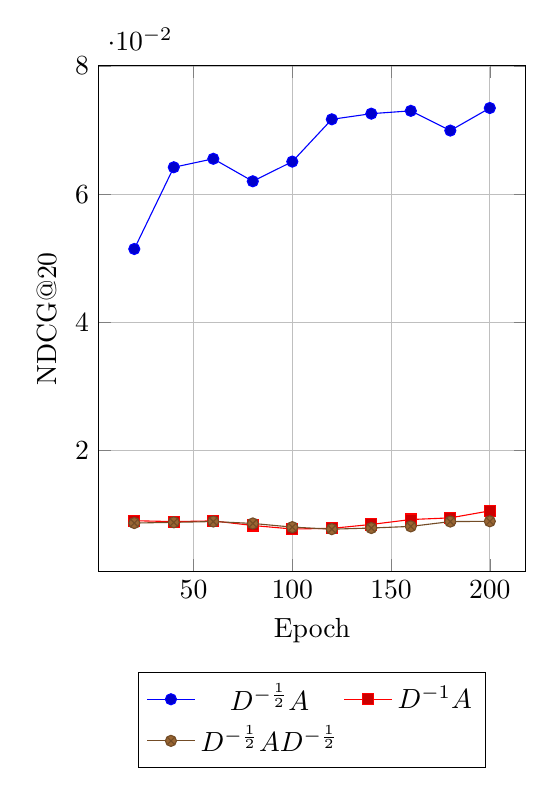
\begin{tikzpicture}
        \begin{axis}[
            xlabel=Epoch,
            ylabel=NDCG@20,
            height=8cm,
            width=7cm,
            grid=major,
            legend style={at={(0.5,-0.20)},
        anchor=north,legend columns=2}]

        \addplot plot coordinates{
            (20,0.05145)
            (40,0.0642)
            (60,0.06552)
            (80,0.06201)
            (100,0.06508)
            (120,0.07168)
            (140,0.07256)
            (160,0.073)
            (180,0.06992)
            (200,0.07344)
        };

        \addplot plot coordinates{
            (20,9.0629e-3)
            (40,8.9258e-3)
            (60,9.0337e-3)
            (80,8.3179e-3)
            (100,7.771e-3)
            (120,7.8698e-3)
            (140,8.4826e-3)
            (160,9.2474e-3)
            (180,9.5092e-3)
            (200,0.0106)
        };

        \addplot plot coordinates{
            (20,8.7e-3)
            (40,8.8121e-3)
            (60,8.9353e-3)
            (80,8.6377e-3)
            (100,8.065e-3)
            (120,7.7449e-3)
            (140,7.9213e-3)
            (160,8.1782e-3)
            (180,8.9256e-3)
            (200,8.9743e-3)
        };

        \legend{$D^{-\frac{1}{2}}A$,$D^{-1}A$,$D^{-\frac{1}{2}}AD^{-\frac{1}{2}}$}
        \end{axis}
    \end{tikzpicture}
    \caption{Effect of various normalizations for CSGCN-ADJ on the Yelp-NC dataset for HR@20.}
    \label{fig:normalization_graph}
\end{figure}
The final embedding matrix after $L$ layers is obtained in the same way as CSGCN-IS where we take the mean of the nodes' representations at each layer.
